As a reminder: the Goddard-Henning conjecture states that every simple triangulated
planar graph of order at least $4$ has total domatic number at least $2$. In this
chapter we try to find (TODO: find a better phrase) equivalent statements to the
conjecture, as well as (hopefully) slightly stronger statements. Even if the stronger
statements are not true, they can be useful for proving the conjecture in special cases.
(e.g. Theorem \ref{thm:odd})

\begin{definition}
  Let $G$ be a triangulated planar graph. For a vertex $v$, each triangle
  containing $v$ has an edge not containing $v$. We call the set of these edges a wheel.
\end{definition}

\begin{figure}[ht]
  \centering
  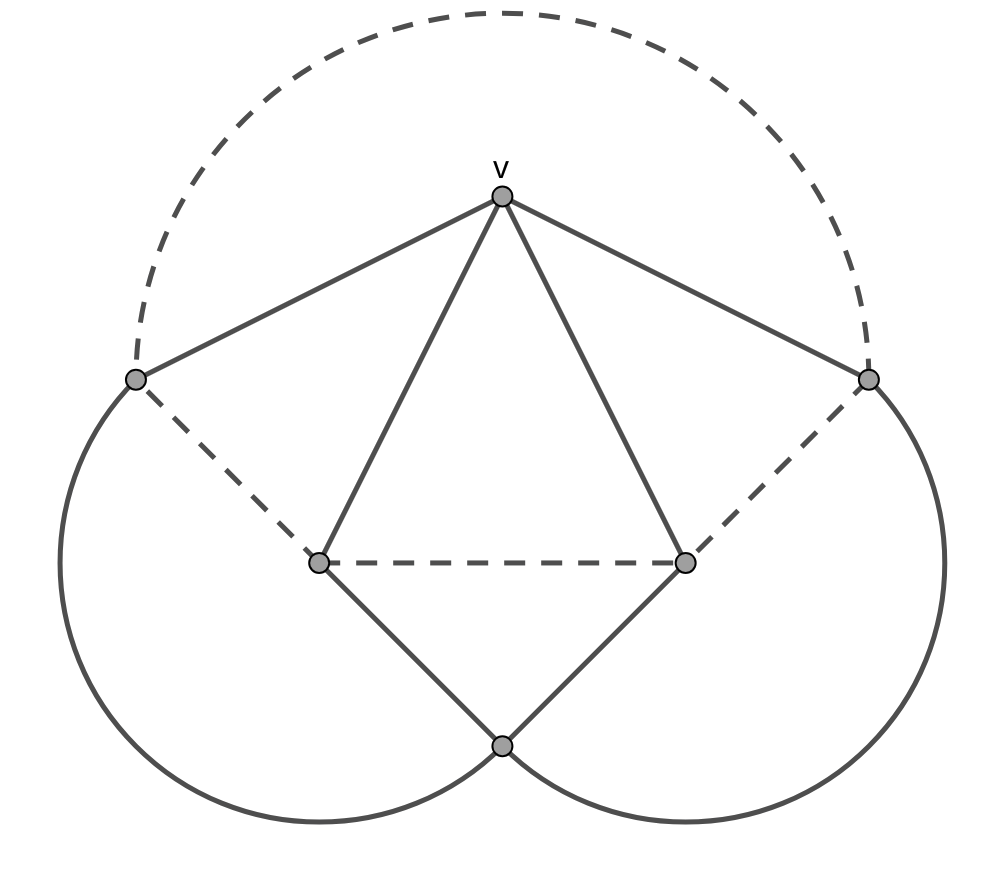
\includegraphics[width=70mm]{wheel}
  \caption{The green edges form the wheel defined by $A$ }
  \label{fig:wheel}
\end{figure}

\begin{guess}\label{s:bipartite}
  Let $G = (V, E)$ be a simple triangulated graph of order at least $4$. Then there
  exists a bipartite $G' = (V, E')$ subgraph of $G$, such that $E'$ contains at
  least one edge from each wheel of $G$.
\end{guess}

\begin{claim}
  The Goddard-Henning conjecture holds if and only if Statement \ref{s:bipartite} holds.
\end{claim}
\begin{proof}
  Let $G$ be a triangulated graph. Suppose first that it has a $2$-coupon coloring.
  $$E' = \{uv \in E\ |\ u\ \textrm{and}\ v\ \textrm{are in different color classes}\}$$
  defines a bipartite subgraph of $G$ that contains at least one edge from each wheel.

  Now suppose that there exists bipartite subgraph that meets our requirement. Color
  the vertices in one of the classes to black, and the vertices in the other class
  to white. This is a $2$-coupon coloring of the original graph.
\end{proof}

\begin{guess}\label{s:forest}
  Let $G = (V, E)$ be a simple triangulated graph of order at least $4$. Then there
  exists a forest in $G$ containing at least one edge from each wheel.
\end{guess}

\begin{remark}
  If Statement \ref{s:forest} holds, then Statement \ref{s:bipartite} also holds.
\end{remark}

\begin{guess}\label{s:no_iso}
  Let $G = (V, E)$ be a simple triangulated graph of order at least $4$. Then there
  exists a subgraph of $G'' = (V, E'')$ having the following two properties.
  \begin{enumerate}
    \item $E""$ contains exactly $1$ edge from each face of $G$.
    \item There are no isolated vertices in $G''$.
  \end{enumerate}
\end{guess}

\begin{lemma}
  A connected planar graph is bipartite if end only if each of its faces have an
  even number of edges.
\end{lemma}
\begin{proof}
  Suppose that the graph is not bipartite and thus there exists a circle $C$ of odd
  length. We show that then exists an odd face. The proof goes by induction on the
  number of faces in the inner side of $C$. If $C$ is a face, then we are done.
  If $C$ is not a face, then there exists a face $F$ in the inner side of $C$ having at least one
  common edge with $C$. $F$ does not contain every edge of $C$, since $G$ is connected.
  Let $C'$ be the symmetric difference of the edge sets of $C$ and $F$. By the parity of $C$
  either $F$ is an odd face or $C'$ is an odd circle containing less faces in its
  inner side than $C$.

  The other direction is trivial.
\end{proof}

\begin{claim}
  If Statement \ref{s:no_iso} holds, then Statement \ref{s:bipartite} (and thus
  the Goddard-Henning conjecture) also holds.
\end{claim}
\begin{proof}
  We show that $G' = (V, E - E'')$ is a subgraph required by Statement \ref{s:bipartite}.
  $G'$ is a bipartite graph, as each of its faces have $4$ edges.
  TBD
\end{proof}

TBD
TODO: Add also a figure about these statements.
